\documentclass[10pt,dvipsnames,table,twocolumn]{article}

% ── Geometry & Encoding ──
\usepackage[utf8]{inputenc}
\usepackage[T1]{fontenc}

% ── Typeface: Palatino + Helvetica condensed for headings ──
\usepackage[sc,osf]{mathpazo}          % Palatino text + math
\usepackage[scaled=0.88]{helvet}       % Helvetica for sans-serif
\usepackage{courier}                   % Courier mono
\linespread{1.08}                      % Palatino needs wider leading

% ── Page geometry ──
\usepackage[
  top=20mm, bottom=20mm,
  left=15mm, right=15mm,
  columnsep=8mm
]{geometry}

% ── Float spacing (more air around tables & figures) ──
\setlength{\textfloatsep}{14pt plus 4pt minus 3pt}
\setlength{\floatsep}{12pt plus 3pt minus 2pt}
\setlength{\intextsep}{12pt plus 3pt minus 2pt}
\setlength{\abovecaptionskip}{8pt}
\setlength{\belowcaptionskip}{4pt}

% ── Maths ──
\usepackage{amsmath, amssymb}

% ── Graphics ──
\usepackage{tikz}
\usetikzlibrary{patterns, arrows.meta, positioning, calc, decorations.pathreplacing, fit}
\usepackage{graphicx}

% ── Tables ──
\usepackage{booktabs}
\usepackage{multirow}
\usepackage{array}
\usepackage{colortbl}

% ── Formatting ──
\usepackage{caption}
\usepackage{subcaption}
\usepackage{enumitem}
\usepackage{titlesec}
\usepackage{fancyhdr}
\usepackage{titling}
\usepackage{needspace}
\usepackage{listings}
\usepackage{xcolor}
\usepackage{float}
\usepackage{dblfloatfix}
\usepackage{microtype}
\usepackage{etoolbox}
\usepackage{tcolorbox}
\tcbuselibrary{skins, breakable}

% ══════════════════════════════════════════════════════════════════
% COLOR PALETTE
% ══════════════════════════════════════════════════════════════════

% ── Ink tones (text, titles, rules) ──
\definecolor{Ink}{HTML}{1A1A2E}            % near-black with blue undertone
\definecolor{DarkInk}{HTML}{16213E}        % deep navy-black for section titles
\definecolor{MidInk}{HTML}{3D4F6F}         % medium for secondary text
\definecolor{LightInk}{HTML}{6B7B99}       % subtle for captions, dates
\definecolor{PaleInk}{HTML}{9AA5B8}        % very light for decorations
\definecolor{Mist}{HTML}{E8ECF1}           % background tint
\definecolor{Snow}{HTML}{F5F7FA}           % code background

% ── Accents (charts, links, highlights) ──
\definecolor{DeepBlue}{HTML}{1B3A6B}       % primary accent
\definecolor{BrightBlue}{HTML}{2E6EC7}     % links, chart line 1
\definecolor{Teal}{HTML}{0E8C7F}           % chart line 2
\definecolor{Coral}{HTML}{C7523B}          % chart line 3 / emphasis
\definecolor{Violet}{HTML}{6C4BA3}         % chart line 4
\definecolor{Gold}{HTML}{C4962C}           % sparingly

% ── Table helpers ──
\definecolor{TableHead}{HTML}{1B3A6B}      % = DeepBlue
\definecolor{TableRowAlt}{HTML}{F2F5F9}    % very subtle alternating

% ══════════════════════════════════════════════════════════════════
% HYPERLINKS
% ══════════════════════════════════════════════════════════════════
\usepackage[
  colorlinks=true,
  linkcolor=DeepBlue,
  urlcolor=BrightBlue,
  citecolor=DeepBlue
]{hyperref}

% ══════════════════════════════════════════════════════════════════
% SECTION STYLING
% ══════════════════════════════════════════════════════════════════

% Section: small-caps, dark, with a thin rule BELOW that doesn't overlap
\titleformat{\section}
  {\needspace{5\baselineskip}\normalsize\sffamily\bfseries\color{DarkInk}}
  {\thesection}
  {0.6em}
  {\MakeUppercase}
\titlespacing*{\section}{0pt}{1.8em}{0.5em}

% Add a thin rule after the section title with proper spacing
\newcommand{\sectionrule}{\vspace{0.2em}\noindent\textcolor{PaleInk}{\rule{\columnwidth}{0.4pt}}\vspace{0.3em}}

% Patch \section to auto-add the rule
\let\oldsection\section
\renewcommand{\section}[1]{\oldsection{#1}\sectionrule}

\titleformat{\subsection}
  {\needspace{8\baselineskip}\small\sffamily\bfseries\color{DarkInk}}
  {\thesubsection}
  {0.5em}
  {}
\titlespacing*{\subsection}{0pt}{1.2em}{0.3em}

\titleformat{\subsubsection}
  {\needspace{5\baselineskip}\small\sffamily\bfseries\itshape\color{MidInk}}
  {\thesubsubsection}
  {0.5em}
  {}
\titlespacing*{\subsubsection}{0pt}{0.9em}{0.2em}

% ══════════════════════════════════════════════════════════════════
% LISTS
% ══════════════════════════════════════════════════════════════════
\setlist{leftmargin=1.5em, itemsep=0.15em, topsep=0.3em, parsep=0.1em}
\setlist[itemize,1]{label={\color{MidInk}\footnotesize$\blacktriangleright$}}
\setlist[itemize,2]{label={\color{LightInk}\textendash}}
\setlist[enumerate,1]{label={\color{MidInk}\arabic*.}}

% ── Paragraphs ──
\setlength{\parskip}{0.4em}
\setlength{\parindent}{0pt}

% ── Default text color ──
\color{Ink}

% ══════════════════════════════════════════════════════════════════
% CAPTIONS
% ══════════════════════════════════════════════════════════════════
\captionsetup{
  font={small},
  labelfont={bf, color=DarkInk, sf},
  textfont={color=MidInk},
  skip=6pt,
  format=hang,
  labelsep=quad
}
\captionsetup[table]{position=above, skip=4pt}
\captionsetup[figure]{position=below}

% ══════════════════════════════════════════════════════════════════
% HEADER / FOOTER
% ══════════════════════════════════════════════════════════════════
\pagestyle{fancy}
\fancyhf{}
\fancyhead[L]{\footnotesize\sffamily\color{LightInk}High-Energy Particle Storms\enspace\textcolor{PaleInk}{|}\enspace HPC Analysis}
\fancyhead[R]{\footnotesize\sffamily\color{LightInk}\thepage}
\renewcommand{\headrulewidth}{0pt}  % no rule — cleaner look

\fancypagestyle{plain}{%
  \fancyhf{}%
  \fancyfoot[C]{\footnotesize\sffamily\color{LightInk}\thepage}%
  \renewcommand{\headrulewidth}{0pt}%
}

% ══════════════════════════════════════════════════════════════════
% TITLE BLOCK
% ══════════════════════════════════════════════════════════════════
\pretitle{\begin{center}\LARGE\sffamily\bfseries\color{DarkInk}}
\posttitle{\end{center}\vspace{0.1em}}
\preauthor{\begin{center}\normalsize\color{MidInk}}
\postauthor{\end{center}}
\predate{\begin{center}\small\color{LightInk}}
\postdate{\end{center}\vspace{-1em}}
\setlength{\droptitle}{-2.5em}

% ══════════════════════════════════════════════════════════════════
% CODE LISTINGS
% ══════════════════════════════════════════════════════════════════
\lstdefinestyle{cstyle}{
  backgroundcolor=\color{Snow},
  basicstyle=\ttfamily\scriptsize\color{Ink},
  keywordstyle=\color{DeepBlue}\bfseries,
  commentstyle=\color{LightInk}\itshape,
  stringstyle=\color{Teal},
  identifierstyle=\color{Ink},
  breaklines=true,
  frame=l,
  framerule=2pt,
  rulecolor=\color{Mist},
  numbers=left,
  numberstyle=\tiny\sffamily\color{PaleInk},
  numbersep=6pt,
  tabsize=4,
  xleftmargin=12pt,
  framexleftmargin=12pt,
  aboveskip=0.8em,
  belowskip=0.6em,
}
\lstset{style=cstyle}

% ── Inline code ──
\let\oldtexttt\texttt
\renewcommand{\texttt}[1]{%
  {\small\colorbox{Mist}{\oldtexttt{\textcolor{DarkInk}{#1}}}}%
}

% ══════════════════════════════════════════════════════════════════
% TABLE STYLING
% ══════════════════════════════════════════════════════════════════
\arrayrulecolor{Mist}
\setlength{\heavyrulewidth}{0.08em}
\setlength{\lightrulewidth}{0.04em}

% ══════════════════════════════════════════════════════════════════
% CUSTOM ENVIRONMENTS
% ══════════════════════════════════════════════════════════════════

% Callout box for key insights
\newtcolorbox{insightbox}[1][]{%
  enhanced,
  colback=Snow,
  colframe=Mist,
  borderline west={2.5pt}{0pt}{DeepBlue},
  sharp corners,
  boxrule=0.4pt,
  left=8pt, right=8pt, top=6pt, bottom=6pt,
  fonttitle=\small\sffamily\bfseries\color{DeepBlue},
  title={#1},
  before skip=0.8em,
  after skip=0.8em,
}

% ══════════════════════════════════════════════════════════════════
% DOCUMENT
% ══════════════════════════════════════════════════════════════════
\title{High-Energy Particle Storms Simulation\\[0.2em]
{\large\color{MidInk} Comparative Analysis of Distributed (MPI/OpenMP) vs.\ GPU (CUDA)}}
\author{Jacopo Mazzatorta}
\date{\today}

\begin{document}

\maketitle
\thispagestyle{plain}

% ══════════════════════════════════════════════════════════════════
\section{Introduction}\label{sec:intro}

The technological development has brought to light many new possibilities and applications in the scientific world.

Real-world phenomena that have always been out of reach in terms of costs and resources are now accessible thanks to High-Performance Computing (HPC) implementations. A relevant example is a high-energy particle storm. Through computational physics, the scientific community can now study radiation and its interactions with the physical world safely.

The goal of this project is to analyze and parallelize a simplified algorithm that simulates the effects of high-energy particle storms on a one-dimensional layer.

As I am not a physicist, the report focuses on the mathematical aspects and the architecture-driven choices of my code implementations, rather than the theoretical physics behind them.

In particular, I present two parallel versions:

\begin{enumerate}
  \item A hybrid \textbf{MPI + OpenMP} version targeting a multi-node CPU cluster.
  \item A \textbf{GPU-accelerated} version using CUDA.
\end{enumerate}

For both versions, I analyze the performance using hardware profilers (\texttt{perf~stat} for CPU, \texttt{nsys} for GPU) to connect the observed speedups to the underlying architecture. Finally, I compare the results to evaluate when each approach is most effective.


% ══════════════════════════════════════════════════════════════════
\section{Test Environment \& Methodology}\label{sec:method}

Before analyzing the results, it is important to define the testing conditions. To ensure a fair comparison between the baseline and the parallel implementations, I followed a strict methodology.

\subsection{Compilation Flags}

All versions of the code were compiled with the highest level of optimization enabled.

\begin{itemize}
  \item \textbf{CPU (GCC):} \texttt{-O3} combined with \texttt{-flto} (Link-Time Optimization) and architecture-specific tuning (\texttt{-march=znver1} for the AMD EPYC Naples nodes). I also enabled aggressive math optimizations (\texttt{-ffinite-math-only}, \texttt{-fno-signed-zeros}) to allow the compiler to vectorize operations that do not require strict IEEE compliance.
  \item \textbf{GPU (NVCC):} \texttt{-O3} with \texttt{-Xptxas~-O3~-Xcompiler~-O3} to target the compute capability of the available GPU.
\end{itemize}

\subsection{Test Cases}

I defined six problem sizes covering a wide range of computational loads. Each test case specifies a layer size, a number of particles, and a number of storm waves.

\begin{table}[t]
\centering
\caption{Test cases used throughout the report.}\label{tbl:testcases}
\small
\begin{tabular}{@{}lrrrl@{}}
\rowcolor{TableHead}
\textcolor{white}{\textbf{Name}} &
\textcolor{white}{\textbf{Layer}} &
\textcolor{white}{\textbf{Particles}} &
\textcolor{white}{\textbf{Waves}} &
\textcolor{white}{\textbf{Used for}} \\
\midrule
test\_02          & 30\,K   & 20\,K & 6 & Strong, Weak, CUDA \\
\rowcolor{TableRowAlt}
personal\_01      & 60\,K   & 20\,K & 6 & Weak prog.\ 1 \\
personal\_02      & 120\,K  & 20\,K & 6 & Strong, Weak, CUDA \\
\rowcolor{TableRowAlt}
test\_07          & 1\,M    & 5\,K  & 4 & Strong, Weak, CUDA \\
personal\_03      & 2\,M    & 5\,K  & 4 & Weak prog.\ 2, CUDA \\
\rowcolor{TableRowAlt}
personal\_04      & 4\,M    & 5\,K  & 4 & Weak prog.\ 2, CUDA \\
\bottomrule
\end{tabular}
\end{table}

\subsection{Baseline}

Measuring speedup requires a fair baseline. Using the original unoptimized sequential code would inflate the results, since the parallel code includes significant algorithmic optimizations (lookup tables, memory alignment, SIMD hints) that have nothing to do with parallelism.

Instead, I used the optimized parallel code compiled with all optimizations enabled, but executed with a single MPI process and a single OpenMP thread. This isolates the speedup that comes purely from parallelism and hardware exploitation.

\begin{insightbox}[Code optimizations alone]
On the 1\,M test, the original sequential code takes 278.8\,s while the optimized single-process baseline takes 7.08\,s---a $39\times$ improvement before any parallelism is applied.
\end{insightbox}

\begin{table}[t]
\centering
\caption{Baseline execution times (optimized code, 1 process, 1 thread). Median of 6 runs.}\label{tbl:baseline}
\small
\begin{tabular}{@{}lrr@{}}
\rowcolor{TableHead}
\textcolor{white}{\textbf{Test Case}} &
\textcolor{white}{\textbf{$T_s$ (s)}} &
\textcolor{white}{\textbf{Range (s)}} \\
\midrule
30\,K    & 1.157  & [1.157,\; 1.159] \\
\rowcolor{TableRowAlt}
60\,K    & 2.293  & [2.289,\; 2.314] \\
120\,K   & 4.621  & [4.613,\; 4.638] \\
\rowcolor{TableRowAlt}
1\,M     & 7.080  & [7.036,\; 7.238] \\
2\,M     & 26.499 & [26.436,\; 26.573] \\
\rowcolor{TableRowAlt}
4\,M     & 58.080 & [57.952,\; 58.125] \\
\bottomrule
\end{tabular}
\end{table}

\subsection{Measurement Protocol}

Each configuration was executed at least 6 times. I report the median execution time and the range (minimum to maximum) as error bars in charts. The median is more robust than the mean against occasional outliers caused by cluster noise.

\subsection{Numerical Validation}

All three versions of the code (baseline, MPI+OpenMP, and CUDA) produce bit-identical results for every test case. The output includes the position and energy value of the maximum after each storm wave, and these match exactly across all configurations and problem sizes. This confirms that the parallelization does not introduce numerical errors.


% ══════════════════════════════════════════════════════════════════
\section{Distributed Memory Parallelization (MPI + OpenMP)}\label{sec:mpi}

The first parallel implementation uses a hybrid approach, combining MPI (Message Passing Interface) with OpenMP. MPI handles communication between different nodes, while OpenMP exploits the cores within each node.

\subsection{Host Architecture \& Setup}

For the experiments, I used the High-Performance Computing cluster of Universit\`a La Sapienza. Each computing node is a dual-socket machine equipped with AMD EPYC Naples processors:

\begin{itemize}
  \item \textbf{Sockets:} 2 per node.
  \item \textbf{Cores:} 16 cores per socket, 32 total per node.
  \item \textbf{Cache:} L1 32\,KB/core, L2 512\,KB/core, L3 8\,MB per CCX (shared by 2 cores). Total L3 per node: 64\,MB.
  \item \textbf{NUMA:} 4 domains per node. Memory is not equally close to all cores.
\end{itemize}

I exploited the NUMA topology by pinning MPI ranks to specific domains using the \texttt{ppr:2:numa} mapping. Each node is organized into 4 NUMA groups:
\begin{equation}
\text{NUMA}_i = \{ \text{node}_{idx} \;|\; idx \pmod{4} = i \}
\end{equation}
By aligning MPI ranks with these physical boundaries, I minimized data movement across the hardware.

\subsection{Implementation \& Optimizations}

\subsubsection{Domain Decomposition}

The core strategy relies on a two-level domain decomposition. At the top level, MPI divides the global layer into equal parts and assigns them to different ranks. At a deeper level, OpenMP divides each rank's section into smaller chunks that individual threads process independently.

Instead of relying on the standard OpenMP scheduler, I used a custom macro to calculate the indices for each thread. This ensures that every thread's partition starts and ends on a cache line boundary (64 bytes = 16 floats), preventing false sharing between cores.

\begin{figure*}[t]
\centering
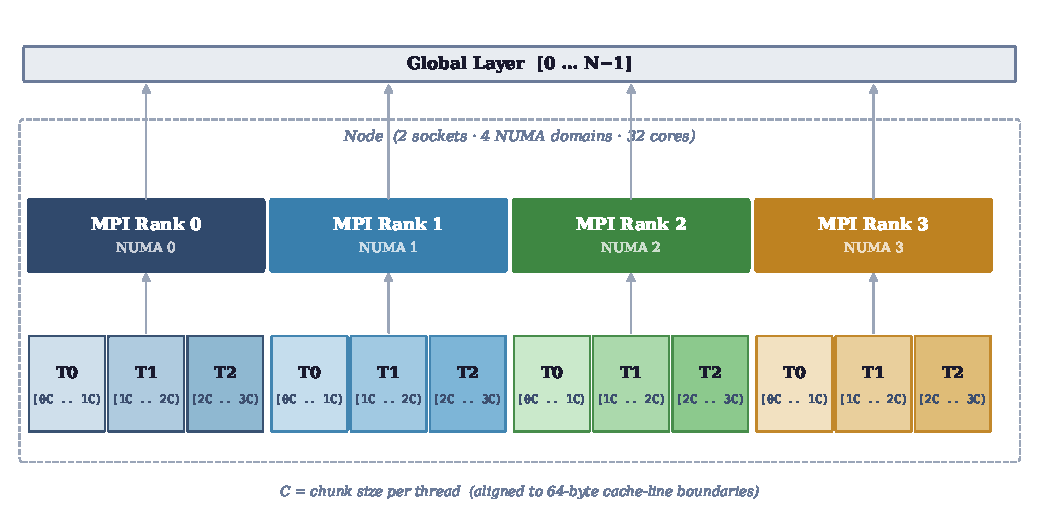
\includegraphics[width=\textwidth]{plots/domain_decomposition.pdf}
\caption{Hybrid domain decomposition: MPI splits the layer across ranks, then OpenMP further partitions each rank's segment among threads with cache-aligned boundaries.}\label{fig:domain-decomp}
\end{figure*}

\subsubsection{Memory Management}

Manually configuring the memory layout was the most effective way to control cache locality and reduce latency. My strategy focuses on three aspects:

\begin{itemize}
  \item \textbf{Alignment:} All memory buffers are aligned to 64 bytes to match the CPU cache line size, preventing false sharing.
  \item \textbf{First-Touch Policy:} I initialize arrays in parallel using the same static chunking logic used for computation. This ensures the OS allocates physical memory on the same socket that will process it.
  \item \textbf{Padding:} Array sizes are rounded up to the next multiple of the SIMD width (16 floats) so that vectorized operations never access invalid memory.
\end{itemize}

\subsubsection{Computational Optimizations}

To speed up the inner particle loop (the bottleneck), I applied several optimizations while preserving numerical correctness.

\begin{itemize}
  \item \textbf{Distance Look-Up Table:} The frequent square root calculations are replaced by a pre-computed table. Since the distances are discrete integers, fetching a value from memory is faster than computing it.
  \item \textbf{Pre-calculated Constants:} In the energy formula, the division by layer size (repeated millions of times) is replaced by a single pre-calculated constant.
  \item \textbf{SIMD Vectorization:} Using \texttt{\#pragma~omp~simd}, the compiler generates AVX2 instructions that process 8 floats simultaneously in 256-bit registers.
\end{itemize}

\subsubsection{Stencil \& Communication}

To avoid slow array copying during relaxation, I use a three-buffer rotation---swapping pointers instead of moving data. For MPI, boundaries are exchanged using non-blocking operations (\texttt{MPI\_Isend}/\texttt{MPI\_Irecv}), allowing the CPU to work on interior cells while border data travels in the background. The global maximum is found using \texttt{MPI\_MAXLOC} to track both the peak energy value and its position.


\subsection{MPI+OpenMP Results}\label{sec:mpi-results}

For all distributed tests, I used the flag \texttt{-{}-map-by~ppr:2:numa:PE=2} to distribute MPI ranks across NUMA domains.

\subsubsection{Strong Scaling}

In strong scaling, the problem size stays fixed while I increase the number of processes. I define speedup as $S_p = T_s / T_p$ and efficiency as $E_p = S_p / p$.

\begin{table}[t]
\centering
\caption{Strong scaling results.}\label{tbl:strong}
\small
\begin{tabular}{@{}llrrrr@{}}
\rowcolor{TableHead}
\textcolor{white}{\textbf{Problem}} &
\textcolor{white}{\textbf{Config}} &
\textcolor{white}{\textbf{Cores}} &
\textcolor{white}{\textbf{Time (s)}} &
\textcolor{white}{\textbf{$S_p$}} &
\textcolor{white}{\textbf{$E_p$}} \\
\midrule
\multirow{3}{*}{30\,K}
  & 1 node  & 32  & 0.233  & 5.0   & 0.155 \\
  & 2 nodes & 64  & 0.041  & 28.3  & 0.443 \\
  & 4 nodes & 128 & 0.022  & 52.4  & 0.410 \\
\midrule
\rowcolor{TableRowAlt}
\multirow{3}{*}{120\,K}
  & 1 node  & 32  & 0.482  & 9.6   & 0.299 \\
\rowcolor{TableRowAlt}
  & 2 nodes & 64  & 0.107  & 43.3  & 0.677 \\
\rowcolor{TableRowAlt}
  & 4 nodes & 128 & 0.053  & 86.6  & 0.676 \\
\midrule
\multirow{3}{*}{1\,M}
  & 1 node  & 32  & 0.565  & 12.5  & 0.391 \\
  & 2 nodes & 64  & 0.121  & 58.5  & 0.913 \\
  & 4 nodes & 128 & 0.070  & 100.5 & 0.785 \\
\bottomrule
\end{tabular}
\end{table}

\begin{figure}[t]
\centering
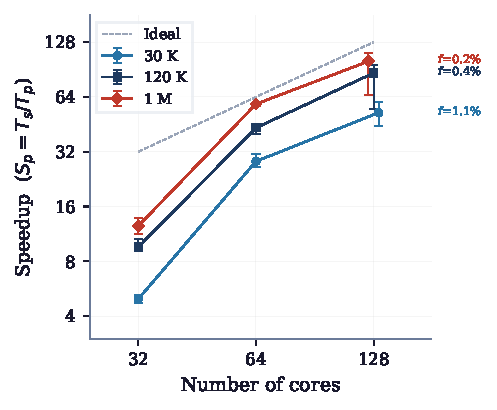
\includegraphics[width=\columnwidth]{plots/strong_scaling.pdf}
\caption{MPI+OpenMP strong scaling: speedup vs.\ number of cores for three problem sizes. The dashed line shows ideal linear scaling.}\label{fig:strong}
\end{figure}

The single-node configuration is significantly slower than expected. On 32 cores, the 1\,M test achieves only $12.5\times$ speedup instead of the theoretical $32\times$. This is caused by thread overcommitment: the configuration uses 16 MPI ranks with 4 OpenMP threads each, producing 64 software threads on 32 physical cores. The excess threads compete for execution resources, causing context switching overhead and cache pollution.

The problem disappears on multi-node runs. The jump from 1 to 2 nodes is much larger than $2\times$: on 30\,K, the 2-node configuration is $5.7\times$ faster than 1-node. This reflects the elimination of overcommitment, not just the addition of hardware.

On 4 nodes (128 cores), the code reaches $100.5\times$ speedup on 1\,M and $86.6\times$ on 120\,K. Using Amdahl's law, the estimated serial fraction is $f = 0.22\%$ for 1\,M, suggesting that the code is highly parallel. The theoretical maximum speedup with infinite cores would be approximately $428\times$.

The 30\,K test scales less efficiently ($52.4\times$ on 128 cores, $f = 1.1\%$) because the problem is too small relative to the communication overhead.


\subsubsection{Weak Scaling}

In weak scaling, I increase the problem size proportionally with the number of nodes. I define weak scaling efficiency as $E_w = T_1 / T_p$. Ideally, $E_w = 1$.

\begin{table}[t]
\centering
\caption{Weak scaling results.}\label{tbl:weak}
\small
\begin{tabular}{@{}llrrr@{}}
\rowcolor{TableHead}
\textcolor{white}{\textbf{Prog.}} &
\textcolor{white}{\textbf{Config}} &
\textcolor{white}{\textbf{Size}} &
\textcolor{white}{\textbf{Time (s)}} &
\textcolor{white}{\textbf{$E_w$}} \\
\midrule
\multirow{3}{*}{1}
  & 1 node  & 30\,K  & 0.233  & 1.00 \\
  & 2 nodes & 60\,K  & 0.060  & 3.86 \\
  & 4 nodes & 120\,K & 0.053  & 4.37 \\
\midrule
\rowcolor{TableRowAlt}
\multirow{3}{*}{2}
  & 1 node  & 1\,M   & 0.565  & 1.00 \\
\rowcolor{TableRowAlt}
  & 2 nodes & 2\,M   & 0.251  & 2.25 \\
\rowcolor{TableRowAlt}
  & 4 nodes & 4\,M   & 0.327  & 1.73 \\
\bottomrule
\end{tabular}
\end{table}

\begin{figure}[t]
\centering
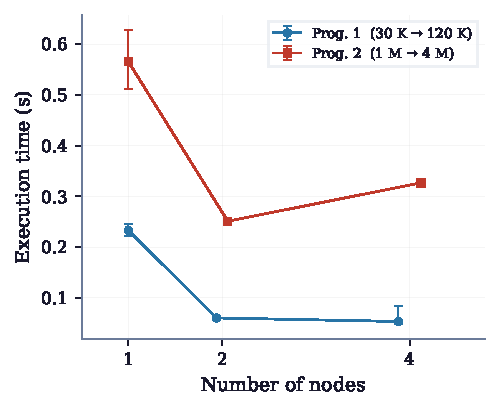
\includegraphics[width=\columnwidth]{plots/weak_scaling.pdf}
\caption{Weak scaling efficiency across 1, 2, and 4 nodes for both problem progressions.}\label{fig:weak}
\end{figure}

Both progressions show super-linear weak efficiency ($E_w > 1$). This is largely an artifact of the 1-node overcommitment: since $T_1$ is inflated, all efficiency values relative to it appear inflated.

Progression~2 shows efficiency degradation at 4 nodes ($E_w$ drops from 2.25 to 1.73). At 4 nodes with a 4\,M layer, the sqrt lookup table grows to 15.6\,MB, which no longer fits in the L3 cache slice of a single CCX (8\,MB on Naples). Since the table is accessed with a random pattern depending on particle positions, this causes cache thrashing. Additionally, the cost of MPI communication grows with the communicator size.


\subsection{CPU Profiling Analysis}\label{sec:cpu-prof}

To understand the performance beyond raw timing, I profiled the 1\,M test using \texttt{perf~stat} in two configurations: the baseline (1~process) and the parallel version (1~node, 32~cores).

\begin{table}[t]
\centering
\caption{Hardware counters from \texttt{perf~stat} on the 1\,M test. Average of 4 runs.}\label{tbl:perf}
\small
\begin{tabular}{@{}lrr@{}}
\rowcolor{TableHead}
\textcolor{white}{\textbf{Metric}} &
\textcolor{white}{\textbf{Baseline}} &
\textcolor{white}{\textbf{Parallel}} \\
\midrule
IPC                     & 1.21          & 1.32 \\
\rowcolor{TableRowAlt}
L1 miss rate            & 13.64\%       & 12.10\% \\
Cache miss rate         & 1.53\%        & 4.06\% \\
\rowcolor{TableRowAlt}
Total instructions      & 24.8\,G       & 39.0\,G \\
Total cycles            & 20.4\,G       & 29.5\,G \\
\rowcolor{TableRowAlt}
Task-clock              & 7.7\,s        & 11.2\,s \\
Wall time               & 7.08\,s       & 0.565\,s \\
\bottomrule
\end{tabular}
\end{table}

The IPC improves from 1.21 to 1.32 because each rank works on a smaller portion of the layer. With 16~MPI ranks on a 1\,M layer, each rank processes 62\,500 floats. The corresponding layer partition (244\,KB) plus the auxiliary array (244\,KB) fit entirely in the L2 cache (512\,KB per core on Naples), reducing memory stalls.

The L1 miss rate drops slightly from 13.64\% to 12.10\%, confirming better data locality per core. However, the overall cache miss rate increases from 1.53\% to 4.06\% because \texttt{perf~stat} measures the entire process tree, including MPI initialization and halo exchanges---operations that generate cache-cold accesses.

The total instruction count grows from 24.8\,G to 39.0\,G, reflecting the overhead of the parallel runtime: OpenMP scheduling, MPI communication, and redundant sqrt table initialization across ranks. The aggregate CPU time is 11.2\,s (vs.\ 7.7\,s baseline), meaning the parallel version uses $1.5\times$ more total CPU work to achieve a $12.5\times$ wall-time improvement.

\begin{figure}[t]
\centering
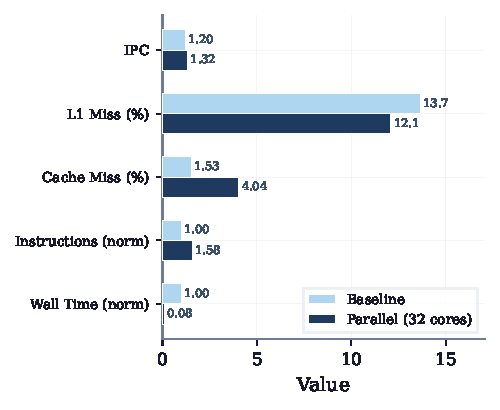
\includegraphics[width=\columnwidth]{plots/perf_comparison.pdf}
\caption{Hardware counter comparison between the baseline (1~process) and the parallel version (1~node, 32~cores) on the 1\,M test.}\label{fig:perf}
\end{figure}


% ══════════════════════════════════════════════════════════════════
\section{GPU Acceleration (CUDA)}\label{sec:cuda}

The second implementation targets the GPU architecture using the NVIDIA CUDA framework.

\subsection{Device Architecture}

I had access to the Quadro RTX 6000 GPU, based on the Turing architecture:

\begin{itemize}
  \item \textbf{CUDA cores:} 4608 (72 SMs, 64 cores/SM).
  \item \textbf{Memory:} 24\,GB GDDR6, 384\,GB/s bandwidth.
  \item \textbf{L2 cache:} 6\,MB.
  \item \textbf{Shared memory:} up to 64\,KB per SM.
  \item \textbf{Peak SP performance:} $\sim$16.3\,TFLOP/s.
\end{itemize}

Threads are grouped into warps of 32, executing the same instruction simultaneously (SIMT model). This is a natural fit for the simulation, where the same energy formula is applied to many data points.

\subsection{Implementation \& Optimizations}

\subsubsection{Domain Decomposition}

Instead of splitting the array into contiguous chunks, I assigned cells using a cyclic pattern:
\begin{equation}
\forall\, i,\quad \text{thread}_i = \{ \text{cell}_j \;|\; j = i + k \cdot N_{\text{threads}},\; j < S_{\text{layer}} \}
\end{equation}
This ensures adjacent threads access adjacent memory addresses, allowing the GPU to coalesce multiple reads into single memory transactions.

\begin{figure*}[t]
\centering
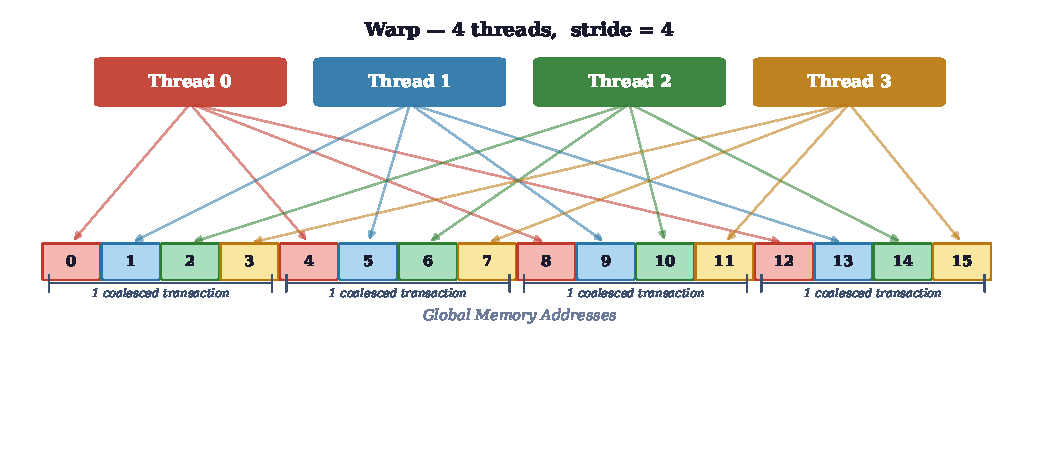
\includegraphics[width=\textwidth]{plots/cuda_coalesced.pdf}
\caption{Coalesced memory access pattern: adjacent threads in a warp access contiguous addresses, enabling efficient memory transactions.}\label{fig:coalesced}
\end{figure*}

\subsubsection{Memory Management}

The most effective optimization was minimizing access to slow global memory by using shared memory. During the stencil phase, threads load a block of the surface into shared memory so that neighbor values can be accessed instantly. For the bombardment phase, I implemented a tiling strategy where threads cooperatively load small chunks of particle data into shared memory.

\subsubsection{Computational Optimizations}

\begin{itemize}
  \item \textbf{Pre-calculated energy scaling:} Instead of dividing energy by the layer size inside the inner loop, I perform this while loading particles into shared memory.
  \item \textbf{Hardware square root:} I use the \texttt{\_\_fsqrt\_rn()} intrinsic to compute square roots directly on the Special Function Units (SFUs). On Turing, each SM has 16~SFUs that can serve a full warp in 2 cycles.
  \item \textbf{Read-only cache:} The \texttt{\_\_ldg()} intrinsic forces particle data through the read-only cache.
  \item \textbf{Loop unrolling:} \texttt{\#pragma~unroll} reduces loop overhead in the inner kernels.
\end{itemize}

\subsubsection{Stencil \& Synchronization}

To avoid array copying during relaxation, I use pointer swapping between two buffers. For the global maximum, I pack both the energy value and its position index into a single 64-bit integer and use \texttt{atomicMax} to find the peak in one hardware-level operation.


\subsection{CUDA Results}\label{sec:cuda-results}

Since there is only one GPU, I measure how the speedup over the baseline changes as the problem size grows.

\begin{table}[t]
\centering
\caption{CUDA performance across problem sizes.}\label{tbl:cuda}
\small
\begin{tabular}{@{}lrrr@{}}
\rowcolor{TableHead}
\textcolor{white}{\textbf{Size}} &
\textcolor{white}{\textbf{$T_s$ (s)}} &
\textcolor{white}{\textbf{CUDA (s)}} &
\textcolor{white}{\textbf{Speedup}} \\
\midrule
30\,K   & 1.157  & 0.021  & 54.9$\times$ \\
\rowcolor{TableRowAlt}
60\,K   & 2.293  & 0.034  & 68.1$\times$ \\
120\,K  & 4.621  & 0.062  & 74.3$\times$ \\
\rowcolor{TableRowAlt}
1\,M    & 7.080  & 0.071  & 99.9$\times$ \\
2\,M    & 26.499 & 0.108  & 245.7$\times$ \\
\rowcolor{TableRowAlt}
4\,M    & 58.080 & 0.211  & 274.6$\times$ \\
\bottomrule
\end{tabular}
\end{table}

The speedup grows from $54.9\times$ on 30\,K to $274.6\times$ on 4\,M. The growth accelerates between 1\,M and 2\,M, where the speedup jumps from $100\times$ to $246\times$, because the CPU and GPU scale differently.

On the CPU, the 2\,M working set (24\,MB across three arrays) exceeds the L3 cache capacity, forcing frequent accesses to slow main memory. On the GPU, the 384\,GB/s bandwidth handles the growth gracefully: the CUDA time increases only $1.5\times$ from 1\,M to 2\,M, while the baseline increases $3.7\times$.

At the small end (30\,K), the GPU is underutilized: only $\sim$59 thread blocks across 72~SMs. At 1\,M, $\sim$1953 blocks fully occupy all SMs---the GPU's sweet spot.

\begin{figure}[t]
\centering
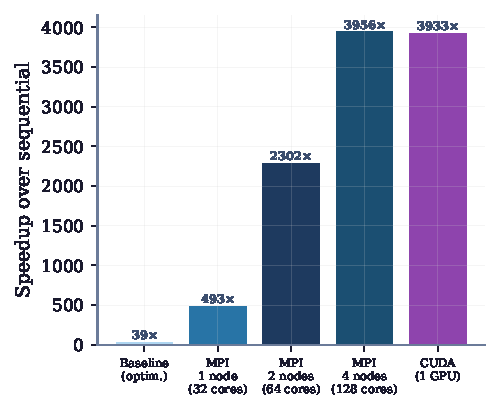
\includegraphics[width=\columnwidth]{plots/speedup_comparison.pdf}
\caption{CUDA speedup over baseline across problem sizes. The dashed line marks $100\times$.}\label{fig:cuda-speedup}
\end{figure}

\begin{figure}[t]
\centering
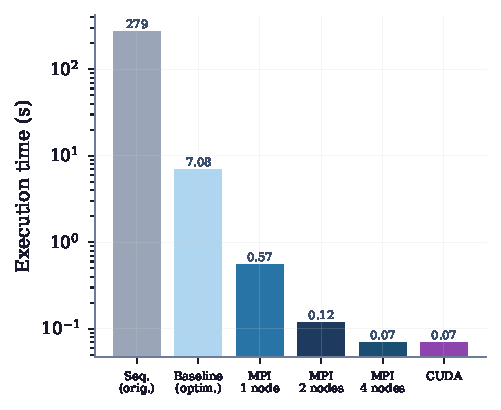
\includegraphics[width=\columnwidth]{plots/time_comparison.pdf}
\caption{Absolute execution time: baseline vs.\ CUDA across problem sizes (log scale).}\label{fig:time-comparison}
\end{figure}


\subsection{GPU Profiling Analysis}\label{sec:gpu-prof}

I profiled the CUDA execution using Nsight Systems (\texttt{nsys}) on the 30\,K and 1\,M tests.

\begin{table}[t]
\centering
\caption{CUDA kernel breakdown from \texttt{nsys}.}\label{tbl:nsys}
\small
\begin{tabular}{@{}llrr@{}}
\rowcolor{TableHead}
\textcolor{white}{\textbf{Test}} &
\textcolor{white}{\textbf{Kernel}} &
\textcolor{white}{\textbf{Time}} &
\textcolor{white}{\textbf{\% GPU}} \\
\midrule
\multirow{3}{*}{30\,K}
  & storm\_kernel      & 19.243\,ms & 99.8\% \\
  & reduce\_max        & 0.018\,ms  & 0.1\% \\
  & stencil            & 0.012\,ms  & 0.1\% \\
\midrule
\rowcolor{TableRowAlt}
\multirow{3}{*}{1\,M}
  & storm\_kernel      & 68.752\,ms & 99.7\% \\
\rowcolor{TableRowAlt}
  & reduce\_max        & 0.128\,ms  & 0.2\% \\
\rowcolor{TableRowAlt}
  & stencil            & 0.068\,ms  & 0.1\% \\
\bottomrule
\end{tabular}
\end{table}

The \texttt{storm\_kernel} dominates completely, accounting for over 99\% of GPU time. The stencil and reduction kernels are negligible because they perform simple operations on contiguous memory with perfect coalesced access.

Memory transfers are also negligible: H2D takes 0.146\,ms on 30\,K (0.8\%) and 0.015\,ms on 1\,M (0.02\%). The particle data is small (${\sim}$160\,KB per storm for 20\,K particles on the 30\,K test, ${\sim}$40\,KB for 5\,K particles on the 1\,M test), the layer is initialized on the GPU via \texttt{cudaMemset}, and only the maximum value and position come back to the host. The implementation is almost purely compute-bound.

The \texttt{storm\_kernel} takes 3.207\,ms per wave on 30\,K and 17.188\,ms per wave on 1\,M---a $5.4\times$ increase for $33\times$ more cells but $4\times$ fewer particles per storm. This sub-linear scaling confirms that 30\,K underutilizes the GPU, while 1\,M reaches higher efficiency.

\begin{figure}[t]
\centering
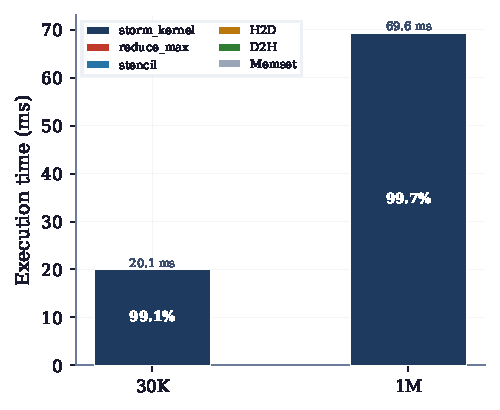
\includegraphics[width=\columnwidth]{plots/cuda_breakdown.pdf}
\caption{GPU time breakdown for the 30\,K and 1\,M tests. The \texttt{storm\_kernel} accounts for over 99\% of execution time in both cases.}\label{fig:cuda-breakdown}
\end{figure}


\subsection{Roofline Analysis}\label{sec:roofline}

To characterize the computational efficiency of the \texttt{storm\_kernel}, I constructed a roofline model for the Quadro RTX~6000. Since the \texttt{ncu} profiler was not accessible due to permission restrictions on the cluster (\texttt{ERR\_NVGPUCTRPERM}), I derived the arithmetic intensity and throughput analytically from the kernel source code and the \texttt{nsys} timing data.

\subsubsection{FLOP Estimation}

The inner loop of the \texttt{storm\_kernel} executes the following operations for each (cell, particle) pair: one subtraction and absolute value for the distance, one addition (\texttt{dist\,+\,1}), one hardware square root (\texttt{\_\_fsqrt\_rn}), one hardware division (\texttt{\_\_fdiv\_rn}), and one accumulation. This amounts to 6 floating-point operations per pair. The total FLOP count for a full run is:
%
\begin{equation}\label{eq:flop}
  \mathrm{FLOP} = S_{\text{layer}} \times N_{\text{particles}} \times 6 \times W
\end{equation}
%
where $W$ is the number of storm waves.

\subsubsection{DRAM Traffic Estimation}

For each \texttt{storm\_kernel} invocation, the minimum DRAM traffic consists of one read and one write of the layer array ($S_{\text{layer}} \times 4 \times 2$~bytes), plus one read of the particle position-value array ($N_{\text{particles}} \times 2 \times 4$~bytes, loaded once into shared memory via tiling). The total bytes over all invocations are:
%
\begin{equation}\label{eq:bytes}
  \mathrm{Bytes} = W \times \bigl( S_{\text{layer}} \times 8 + N_{\text{particles}} \times 8 \bigr)
\end{equation}
%
This is a lower bound: L2 misses and replay transactions may increase the actual DRAM traffic, but the tiling strategy keeps particle data in shared memory and the layer access pattern is fully coalesced, so the estimate is reasonable.

\subsubsection{Results}

\begin{table}[t]
\centering
\caption{Roofline model results for \texttt{storm\_kernel} (analytical).}\label{tbl:roofline}
\small
\begin{tabular}{@{}lrrrrr@{}}
\rowcolor{TableHead}
\textcolor{white}{\textbf{Test}} &
\textcolor{white}{\textbf{FLOP (G)}} &
\textcolor{white}{\textbf{Bytes (MB)}} &
\textcolor{white}{\textbf{AI (F/B)}} &
\textcolor{white}{\textbf{GF/s}} &
\textcolor{white}{\textbf{\% Peak}} \\
\midrule
30\,K  & 21.6  & 2.4   & ${\sim}$9\,000  & 1\,123 & 6.9\%  \\
\rowcolor{TableRowAlt}
1\,M   & 120.0 & 32.2  & ${\sim}$3\,750  & 1\,745 & 10.7\% \\
\bottomrule
\end{tabular}
\end{table}

Both points fall deep in the compute-bound region of the roofline (Figure~\ref{fig:roofline}). With arithmetic intensities of 3\,750--9\,000\,FLOP/byte, the kernel is far above the ridge point ($\approx 42$\,FLOP/byte for DRAM, $\approx 8$\,FLOP/byte for L2), meaning that performance is limited by compute throughput, not memory bandwidth.

The achieved throughput of 1.1--1.7\,TFLOP/s represents 6.9--10.7\% of the 16.3\,TFLOP/s FP32 peak. This gap is expected for a kernel dominated by high-latency special function unit (SFU) operations: each \texttt{\_\_fsqrt\_rn} and \texttt{\_\_fdiv\_rn} is dispatched to one of the 16~SFUs per SM, which can serve a full warp in 2~cycles---significantly slower than the 64~FP32 CUDA cores that can retire a full warp every cycle. The inner loop's data dependency chain (distance $\to$ sqrt $\to$ division $\to$ accumulation) further limits instruction-level parallelism.

The 1\,M test achieves higher throughput than 30\,K (1\,745 vs.\ 1\,123\,GFLOP/s) because the larger grid (1\,953 vs.\ 59~blocks) provides enough warps to keep all 72~SMs occupied and hide the SFU latency through thread-level parallelism.

\begin{figure}[t]
\centering
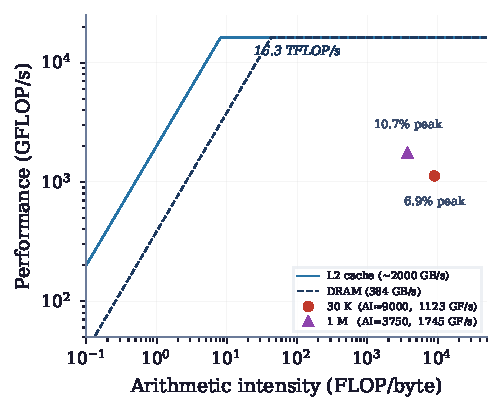
\includegraphics[width=\columnwidth]{plots/roofline.pdf}
\caption{Roofline model for the Quadro RTX~6000. Both kernel configurations fall in the compute-bound region, reaching 6.9--10.7\% of peak FP32 throughput.}\label{fig:roofline}
\end{figure}


% ══════════════════════════════════════════════════════════════════
\section{Final Comparison \& Conclusion}\label{sec:comparison}

\begin{table}[t]
\centering
\caption{Direct comparison on shared problem sizes.}\label{tbl:comparison}
\small
\begin{tabular}{@{}lrrrr@{}}
\rowcolor{TableHead}
\textcolor{white}{\textbf{Size}} &
\textcolor{white}{\textbf{MPI best}} &
\textcolor{white}{\textbf{CUDA}} &
\textcolor{white}{\textbf{MPI $S_p$}} &
\textcolor{white}{\textbf{CUDA $S_p$}} \\
\midrule
30\,K   & 0.022\,s  & 0.021\,s  & 52.4$\times$  & 54.9$\times$  \\
\rowcolor{TableRowAlt}
120\,K  & 0.053\,s  & 0.062\,s  & 86.6$\times$  & 74.3$\times$  \\
1\,M    & 0.070\,s  & 0.071\,s  & 100.5$\times$ & 99.9$\times$  \\
\rowcolor{TableRowAlt}
2\,M    & 0.251\,s  & 0.108\,s  & 105.6$\times$ & 245.7$\times$ \\
4\,M    & 0.327\,s  & 0.211\,s  & 177.3$\times$ & 274.6$\times$ \\
\bottomrule
\end{tabular}
\end{table}

On the small test (30\,K), one GPU and a 128-core cluster achieve nearly identical performance (${\sim}$21\,ms). On 120\,K, the MPI cluster is slightly faster (53\,ms vs.\ 62\,ms) because domain decomposition allows each rank's working set to fit entirely in L2 cache. On 1\,M, the two approaches are tied (${\sim}$71\,ms).

The divergence starts at larger problems. On 2\,M, CUDA is $2.3\times$ faster (108\,ms vs.\ 251\,ms). On 4\,M, CUDA is $1.5\times$ faster (211\,ms vs.\ 327\,ms). The CPU baseline degrades super-linearly above 1\,M due to L3 cache overflow, while the GPU's DRAM bandwidth handles the additional data without significant penalty.

\begin{figure}[t]
\centering
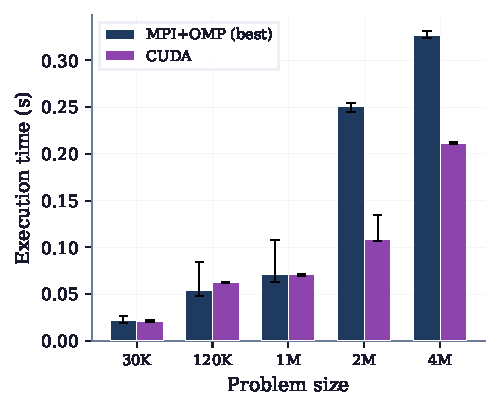
\includegraphics[width=\columnwidth]{plots/mpi_vs_cuda.pdf}
\caption{Execution time comparison between best MPI configuration (128~cores, 4~nodes) and CUDA across problem sizes.}\label{fig:mpi-vs-cuda}
\end{figure}

Both approaches achieve strong speedups but for different architectural reasons. The MPI+OpenMP version exploits domain decomposition to keep per-rank data in fast cache, combined with NUMA-aware placement to minimize memory latency. The CUDA version exploits massive thread-level parallelism and high memory bandwidth to hide latency.

In practice, if the simulation fits on one GPU, CUDA is the simpler and more cost-effective choice---one graphics card matches a 128-core cluster. For problems exceeding GPU memory (24\,GB on the RTX~6000), MPI across multiple nodes remains the only option.


\subsection{Limitations and Future Work}

This study is limited to a single GPU and a maximum of 4 compute nodes. The 1-node MPI results are affected by thread overcommitment, which inflates the weak scaling efficiency values. The \texttt{ncu} profiler was not accessible due to permission restrictions on the cluster, preventing hardware-counter-based occupancy and throughput measurements; the roofline model was therefore constructed analytically from the kernel source code, which provides a lower bound on DRAM traffic and may slightly overestimate the arithmetic intensity. Natural extensions would include multi-GPU configurations, hybrid MPI+CUDA for problems exceeding single-GPU memory, and mixed-precision computation.

\end{document}
